\begin{wrapfigure}[0]{r}[-1cm]{4cm}
 \vspace{-6cm}
  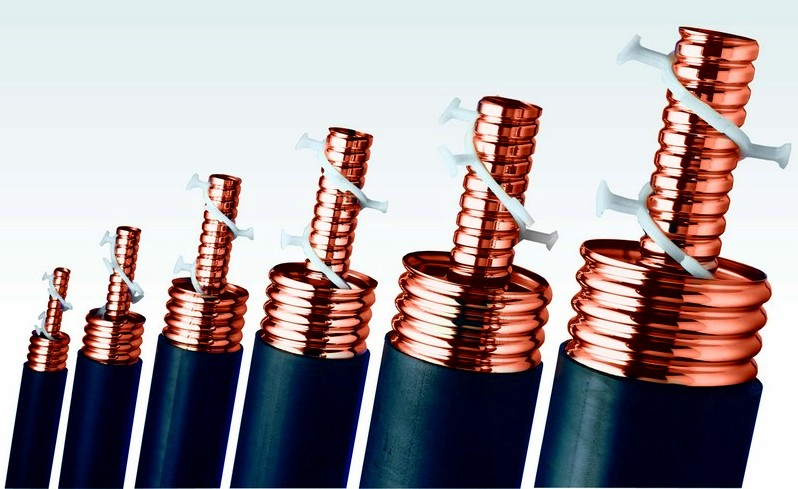
\includegraphics[scale=0.2]{DDK/Bilder/Cables.jpg}
 \vspace{-6cm}
\end{wrapfigure}

\section*{Theorie- und Prüfungsfragen}

~~~~~~
\subsection*{Die Dämpfung}

\begin{enumerate} 
\itemsep1pt\parskip0pt\parsep0pt
\item[1] Was wird unter dem Ausdruck Dämpfungsfaktor verstanden?
\loesung{Das Verhältnis von der am Anfang einer Übertragungsstrecke vorhandenen Leistung $P_1$ zu der am Ende übrig gebliebenen Leistung $P_2$ wird als Dämpfungsfaktor $D$ bezeichnet. $D_P = \dfrac{P_1}{P_2}$ }
\item[2] Was wird unter dem Ausdruck Verstärkungsfaktor verstanden?
\loesung{Das Verhältnis von der am Ende einer Übertragungsstrecke erreichten Leistung $P_2$ zu der am Eingang vorhandenen Leistung $P_1$ wird als Verstärkungsfaktor $T$ bezeichnet. $T = \dfrac{P_2}{P_1}$ }
\item[3] Zur besseren Handhabung ist es möglich die Dämpfung und die Verstärkung in $dB$ anzugeben. Wie lässt sich das berechnen?
\loesung{$a_p = 10 \cdot lg \dfrac{P_1}{P_2}$; $g=10 \cdot lg \dfrac{P_2}{P_1} $}
\item[4] Am Eingang bzw. am Ausgang einer Übertragungsstrecke liegen verschiedene Leistungen an. Berechne jeweils die fehlenden Einträge.
\end{enumerate}

\begin{figure}[H]
	\subfigure{
		\begin{tabular}{|l|l|l|l|}
			\hline
			Eingang & Ausgang & Dämpfung & Verstärkung\\
			\hline
			$1W$ & $4W$ &  & ~\hspace*{1cm}\\
			$4W$ & $1W$ &  & ~\hspace*{1cm}\\
			$4W$ & $10W$ &  & ~\hspace*{1cm}\\
			$50W$ &  & $-7dB$ & \\
			\hline
		\end{tabular}
	}
	\subfigure{
		\loesung{
			\begin{tabular}{|l|l|l|l|}
				\hline
				Eingang & Ausgang & Dämpfung & Verstärkung\\
				\hline
				$1W$ & $4W$ & $-6dB$ & $6dB$\\
				$4W$ & $1W$ & $6dB$ & $-6dB$\\
				$4W$ & $10W$ & $-4dB$ & $4dB$\\
				$50W$ & $20W$  & $-7dB$ & $7dB$\\
				\hline
			\end{tabular}
			}
	}
\end{figure}

\subsection*{S-Stufen}

\begin{enumerate} 
\itemsep1pt\parskip0pt\parsep0pt
\item[5] Zur Angabe der Empfangsfeldstärke wurde im RST-System für die Lautstärke $S9$ ein bestimmter Wert einer Empfangsspannung an einem $50\Omega$-Eingang für KW und UKW festgelegt. Wie lautet diese Angabe?
\loesung{KW: $S9 \hat{=} 50\mu V ~an~ 50\Omega$; UKW: $S9 \hat{=} 5\mu V ~an~ 50\Omega$}
\item[6] Die Erhöhung der Sendeleistung um eine S-Stufe entspricht einer Erhöhung um wie viel $dB$?
\item[7] Die Erhöhung der Sendeleistung um eine S-Stufe entspricht einer Erhöhung der Empfangsspannung um wie viel $\mu V$?
\item[8] \emph{\textbf{TITF406}} Wie groß ist der Unterschied von S4 nach S7 in dB?
	\begin{enumerate}
	\itemsep1pt\parskip0pt\parsep0pt
		\item[A] 3 dB
		\item[B] 9 dB
		\item[C] 18 dB
		\item[D] 24 dB
		\loesung{Lösung C}
	\end{enumerate}
\item[9] \emph{\textbf{TI403}} Um wie viel S-Stufen müsste die S-Meter-Anzeige Ihres Empfängers steigen, wenn Ihr Partner die Sendeleistung von 10 Watt auf 40 Watt erhöht? Um ...
	\begin{enumerate}
	\itemsep1pt\parskip0pt\parsep0pt
		\item[A] eine S-Stufe
		\item[B] zwei S-Stufen
		\item[C] vier S-Stufen
		\item[D] acht S-Stufen
		\loesung{Lösung A}
	\end{enumerate}
\item[10] \emph{\textbf{TI404}} Ein Funkamateur kommt laut S-Meter mit S7 an. Dann schaltet er seine Endstufe ein und bittet um einen erneuten Rapport. Das S-Meter zeigt S9+8dB. Um welchen Faktor müsste der Funkamateur seine Leistung erhöht haben?
	\begin{enumerate}
	\itemsep1pt\parskip0pt\parsep0pt
		\item[A] 120-fach
		\item[B] 20-fach 
		\item[C] 10-fach
		\item[D] 100-fach
		\loesung{Lösung D}
	\end{enumerate}
\end{enumerate}

\subsection*{Pegel}

\begin{enumerate} 
\itemsep1pt\parskip0pt\parsep0pt
\item[11] Wie lautet die Formel für den Leistungspegel (dBmW)?
\loesung{$p=10\cdot lg\dfrac{P}{1mW}$}
\item[12] \emph{\textbf{TH304}}  Welcher der nachfolgenden Zusammenhänge ist richtig?
	\begin{enumerate}
	\itemsep1pt\parskip0pt\parsep0pt
		\item[A] 	0 dBm entspricht 1 mW;
					3 dBm entspricht 1,4 mW;
					20 dBm entspricht 10 mW
		\item[B] 	0 dBm entspricht 0 mW;
					3 dBm entspricht 30 mW;
					20 dBm entspricht 200 mW
		\item[C] 	1 dBm entspricht 0 mW;
					2 dBm entspricht 3 mW;
					100 dBm entspricht 20 mW
		\item[D] 	0 dBm entspricht 1 mW;
					3 dBm entspricht 2 mW;
					20 dBm entspricht 100 mW
		\loesung{Lösung D}
	\end{enumerate}
\end{enumerate}

\subsection*{Wellenwiderstand}

\begin{enumerate} 
\itemsep1pt\parskip0pt\parsep0pt
\item[13] Wie lässt sich der Wellenwiderstand einer Leitung berechnen?
\loesung{aus dem Kapazitätsbelag $C'$ (C pro m) und dem Induktivitätsbelag $L'$ (L pro m) $ Z_w = \sqrt{ \dfrac{L'}{C'} } $}
\item[14] \emph{\textbf{TH307}}  Der Wellenwiderstand einer Leitung
	\begin{enumerate}
	\itemsep1pt\parskip0pt\parsep0pt
		\item[A] ist völlig frequenzunabhängig.
		\item[B] hängt von der Beschaltung am Leitungsende ab.
		\item[C] hängt von der Leitungslänge und der Beschaltung am Leitungsende ab.
		\item[D] ist im HF-Bereich in etwa konstant und unabhängig vom Leitungsabschluss.
		\loesung{Lösung D}
	\end{enumerate}
\item[14] \emph{\textbf{TH308}}  Koaxialkabel weisen typischerweise Wellenwiderstände von
	\begin{enumerate}
	\itemsep1pt\parskip0pt\parsep0pt
		\item[A] 50, 300 und 600 Ohm auf.
		\item[B] 60, 120 und 240 Ohm auf.
		\item[C] 50, 60 und 75 Ohm auf.
		\item[D] 50, 75 und 240 Ohm auf.
		\loesung{Lösung C}
	\end{enumerate}
\item[15] \emph{\textbf{TH309}}  Welche Vorteile hat eine Paralleldraht-Speiseleitung gegenüber der Speisung über ein Koaxialkabel?
	\begin{enumerate}
	\itemsep1pt\parskip0pt\parsep0pt
		\item[A] Sie vermeidet Mantelwellen durch Wegfall der Abschirmung.
		\item[B] Sie erlaubt leichtere Kontrolle des Wellenwiderstandes durch Verschieben der Spreizer.
		\item[C] Sie bietet guten Blitzschutz durch niederohmige Drähte.
		\item[D] Sie hat geringere Dämpfung und hohe Spannungsfestigkeit.
		\loesung{Lösung D}
	\end{enumerate}
\end{enumerate}

\subsection*{Dämpfungsberechnung}

\begin{enumerate} 
\itemsep1pt\parskip0pt\parsep0pt
\item[16] \emph{\textbf{TH306}}  Welche Dämpfung hat ein 20 m langes Koaxkabel vom Typ RG58 bei 29 MHz? (siehe hierzu Diagramm ...)
	\begin{enumerate}
	\itemsep1pt\parskip0pt\parsep0pt
		\item[A] 4,5 dB
		\item[B] 1,8 dB
		\item[C] 9,0 dB
		\item[D] 1,2 dB
		\loesung{Lösung B}
	\end{enumerate}
\item[17] \emph{\textbf{TH305}}  Welche Dämpfung hat ein 25 m langes Koaxkabel vom Typ Aircell 7 bei 145 MHz? (siehe hierzu Diagramm)
	\begin{enumerate}
	\itemsep1pt\parskip0pt\parsep0pt
		\item[A] 1,9 dB
		\item[B] 7,5 dB
		\item[C] 3,75 dB
		\item[D] 1,5 dB
		\loesung{Lösung A}
	\end{enumerate}
\item[18] \emph{\textbf{TH302}}  Am Ende einer Leitung ist nur noch ein Zehntel der Leistung vorhanden. Wie groß ist das Dämpfungsmaß des Kabels?
	\begin{enumerate}
	\itemsep1pt\parskip0pt\parsep0pt
		\item[A] 16 dB
		\item[B] 3 dB
		\item[C] 6 dB
		\item[D] 10 dB
		\loesung{Lösung A}
	\end{enumerate}
\end{enumerate}

\subsection*{Stehwellenverhältnis und Symmetrierung}

\begin{enumerate} 
\itemsep1pt\parskip0pt\parsep0pt
\item[19] Was wird unter dem Ausdruck Stehwellenverhältnis verstanden und wie wird es berechnet?
\loesung{Wie gut Antennen und die jeweilige Zuleitung aneinander angepasst sind, kann mit dem Stehwellenverhältnis beschrieben werden. $ SWR = \dfrac{U_{max}}{U_{min}} = \dfrac{u_h + u_r}{u_h - u_r} $}
\item[20] \emph{\textbf{TH403}}  Welche Auswirkungen hat es, wenn eine symmetrische Antenne (Dipol) mit einem Koaxkabel gleicher Impedanz gespeist wird?
	\begin{enumerate}
	\itemsep1pt\parskip0pt\parsep0pt
		\item[A] Es treten keine nennenswerten Auswirkungen auf, da die Antenne angepasst ist und die Speisung über ein Koaxkabel erfolgt, dessen Außenleiter Erdpotential hat.
		\item[B] Die Richtcharakteristik der Antenne wird verformt und es können Mantelwellen auftreten.
		\item[C] Am Speisepunkt der Antenne treten gegenphasige Spannungen und Ströme gleicher Größe auf, die eine Fehlanpassung hervorrufen.
		\item[D] Es treten Polarisationsdrehungen auf, die von der Kabellänge abhängig sind.
		\loesung{Lösung B}
	\end{enumerate}
\item[21] \emph{\textbf{TH310}}  Wann ist eine Speiseleitung unsymmetrisch? Sie ist unsymmetrisch, wenn ...
	\begin{enumerate}
	\itemsep1pt\parskip0pt\parsep0pt
		\item[A] die hin- und zurücklaufende Leistung verschieden sind.
		\item[B] sie außerhalb ihrer Resonanzfrequenz betrieben wird.
		\item[C] die beiden Leiter unterschiedlich geformt sind, z.B. Koaxialkabel.
		\item[D] die Koaxial-Leitung Spannung gegen Erde führt.
		\loesung{Lösung C}
	\end{enumerate}
\item[22] \emph{\textbf{TH405}}  Auf einem Ferritkern sind etliche Windungen Koaxial-kabel aufgewickelt. Diese Anordnung kann dazu dienen, ...
	\begin{enumerate}
	\itemsep1pt\parskip0pt\parsep0pt
		\item[A] statische Aufladungen zu verhindern.
		\item[B] eine Antennenleitung abzustimmen.
		\item[C] Mantelwellen zu dämpfen.
		\item[D] Oberwellen zu unterdrücken.
		\loesung{Lösung C}
	\end{enumerate}
\end{enumerate}

